

\tikzset{every picture/.style={line width=0.75pt}} %set default line width to 0.75pt        

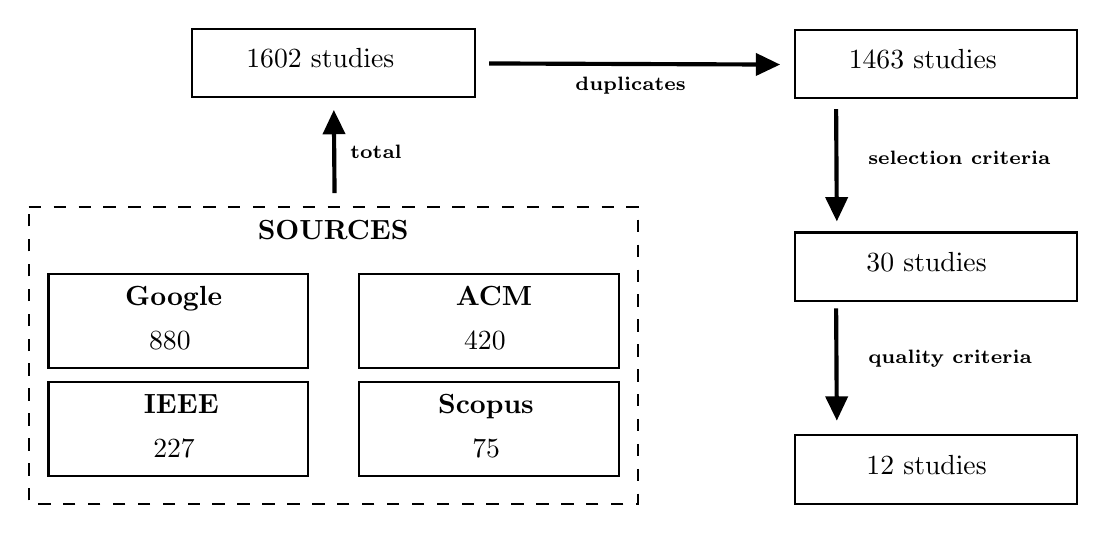
\begin{tikzpicture}[x=0.75pt,y=0.75pt,yscale=-1,xscale=1]
%uncomment if require: \path (0,300); %set diagram left start at 0, and has height of 300

%Shape: Rectangle [id:dp6546352297933162] 
\draw   (17.04,127.79) -- (141.98,127.79) -- (141.98,173.01) -- (17.04,173.01) -- cycle ;

%Shape: Rectangle [id:dp8303551301255043] 
\draw   (166.79,127.79) -- (291.72,127.79) -- (291.72,173.01) -- (166.79,173.01) -- cycle ;

%Shape: Rectangle [id:dp8113957066476918] 
\draw   (17.04,179.76) -- (141.98,179.76) -- (141.98,224.98) -- (17.04,224.98) -- cycle ;

%Shape: Rectangle [id:dp25742759249794456] 
\draw   (166.79,179.76) -- (291.72,179.76) -- (291.72,224.98) -- (166.79,224.98) -- cycle ;


%Shape: Rectangle [id:dp887698650238713] 
\draw  [dash pattern={on 4.5pt off 4.5pt}] (7.5,95.27) -- (301.26,95.27) -- (301.26,238.27) -- (7.5,238.27) -- cycle ;


%Shape: Rectangle [id:dp2249952504303483] 
\draw   (86.25,9.5) -- (222.51,9.5) -- (222.51,42.35) -- (86.25,42.35) -- cycle ;

%Shape: Rectangle [id:dp5429657438012057] 
\draw   (376.5,10) -- (512.76,10) -- (512.76,42.85) -- (376.5,42.85) -- cycle ;

%Shape: Rectangle [id:dp8170922890561967] 
\draw   (376.5,107.7) -- (512.76,107.7) -- (512.76,140.56) -- (376.5,140.56) -- cycle ;

%Shape: Rectangle [id:dp9256107502869182] 
\draw   (376.5,205.42) -- (512.76,205.42) -- (512.76,238.27) -- (376.5,238.27) -- cycle ;

%Straight Lines [id:da1413992770510486] 
\draw [line width=1.5]    (154.85,88.74) -- (154.55,52.74) ;
\draw [shift={(154.51,48.74)}, rotate = 449.52] [fill={rgb, 255:red, 0; green, 0; blue, 0 }  ][line width=0.08]  [draw opacity=0] (11.61,-5.58) -- (0,0) -- (11.61,5.58) -- cycle    ;
%Straight Lines [id:da8404466389733534] 
\draw [line width=1.5]    (229.35,26.24) -- (365.43,26.76) ;
\draw [shift={(369.43,26.77)}, rotate = 180.22] [fill={rgb, 255:red, 0; green, 0; blue, 0 }  ][line width=0.08]  [draw opacity=0] (11.61,-5.58) -- (0,0) -- (11.61,5.58) -- cycle    ;

%Straight Lines [id:da5612249585170423] 
\draw [line width=1.5]    (396.82,98.24) -- (396.51,48.24) ;
\draw [shift={(396.85,102.24)}, rotate = 269.65] [fill={rgb, 255:red, 0; green, 0; blue, 0 }  ][line width=0.08]  [draw opacity=0] (11.61,-5.58) -- (0,0) -- (11.61,5.58) -- cycle    ;

%Straight Lines [id:da8483032617409181] 
\draw [line width=1.5]    (396.82,194.24) -- (396.51,144.24) ;
\draw [shift={(396.85,198.24)}, rotate = 269.65] [fill={rgb, 255:red, 0; green, 0; blue, 0 }  ][line width=0.08]  [draw opacity=0] (11.61,-5.58) -- (0,0) -- (11.61,5.58) -- cycle    ;


% Text Node
\draw (203.26,184.17) node [anchor=north west][inner sep=0.75pt]   [align=left] {\textbf{Scopus}};
% Text Node
\draw (219.76,205.8) node [anchor=north west][inner sep=0.75pt]   [align=left] {75};
% Text Node
\draw (211.76,132.2) node [anchor=north west][inner sep=0.75pt]   [align=left] {\textbf{ACM}};
% Text Node
\draw (215.76,153.83) node [anchor=north west][inner sep=0.75pt]   [align=left] {420};
% Text Node
\draw (52.51,132.2) node [anchor=north west][inner sep=0.75pt]   [align=left] {\textbf{Google }};
% Text Node
\draw (64.01,153.83) node [anchor=north west][inner sep=0.75pt]   [align=left] {880 };
% Text Node
\draw (61.51,184.17) node [anchor=north west][inner sep=0.75pt]   [align=left] {\textbf{IEEE}};
% Text Node
\draw (66.01,205.8) node [anchor=north west][inner sep=0.75pt]   [align=left] {227};
% Text Node
\draw (116.38,100.24) node [anchor=north west][inner sep=0.75pt]   [align=left] {\textbf{SOURCES}};
% Text Node
\draw (110.88,17.43) node [anchor=north west][inner sep=0.75pt]   [align=left] {1602 studies};
% Text Node
\draw (401.13,17.93) node [anchor=north west][inner sep=0.75pt]   [align=left] {1463 studies};
% Text Node
\draw (409.63,115.63) node [anchor=north west][inner sep=0.75pt]   [align=left] {30 studies};
% Text Node
\draw (409.63,213.34) node [anchor=north west][inner sep=0.75pt]   [align=left] {12 studies};
% Text Node
\draw (161,64.25) node [anchor=north west][inner sep=0.75pt]   [align=left] {{\scriptsize \textbf{total}}};
% Text Node
\draw (410.5,66.74) node [anchor=north west][inner sep=0.75pt]   [align=left] {{\scriptsize \textbf{selection criteria}}};
% Text Node
\draw (410.5,162.74) node [anchor=north west][inner sep=0.75pt]   [align=left] {{\scriptsize \textbf{quality criteria}}};
% Text Node
\draw (269.39,31.25) node [anchor=north west][inner sep=0.75pt]   [align=left] {{\scriptsize \textbf{duplicates}}};


\end{tikzpicture}
